%%%%%%%%%%%%%%%%%%%%%%%%%%%%%%%%%%%%%%%%%
% Short Sectioned Assignment
% LaTeX Template
% Version 1.0 (5/5/12)
%
% This template has been downloaded from:
% http://www.LaTeXTemplates.com
%
% Original author:

% Frits Wenneker (http://www.howtotex.com)
%
% License:
% CC BY-NC-SA 3.0 (http://creativecommons.org/licenses/by-nc-sa/3.0/)
%
%%%%%%%%%%%%%%%%%%%%%%%%%%%%%%%%%%%%%%%%%

%----------------------------------------------------------------------------------------
%	PACKAGES AND OTHER DOCUMENT CONFIGURATIONS
%----------------------------------------------------------------------------------------

\documentclass[paper=a4, fontsize=11pt]{scrartcl} % A4 paper and 11pt font size

\usepackage[T1]{fontenc} % Use 8-bit encoding that has 256 glyphs
\usepackage{fourier} % Use the Adobe Utopia font for the document - comment this line to return to the LaTeX default
\usepackage[english]{babel} % English language/hyphenation
\usepackage{amsmath,amsfonts,amsthm} % Math packages

\usepackage{lipsum} % Used for inserting dummy 'Lorem ipsum' text into the template

\usepackage{enumitem}
\usepackage{mathtools}
\DeclarePairedDelimiter\ceil{\lceil}{\rceil}
\DeclarePairedDelimiter\floor{\lfloor}{\rfloor}
\usepackage{graphicx}
\usepackage{subfig}	
\usepackage{listings}
\usepackage{amsmath}
\usepackage{algorithm}
\usepackage[noend]{algpseudocode}
\makeatletter
\def\BState{\State\hskip-\ALG@thistlm}
\makeatother

\usepackage{sectsty} % Allows customizing section commands
\allsectionsfont{\centering \normalfont\scshape} % Make all sections centered, the default font and small caps

\usepackage{fancyhdr} % Custom headers and footers
\pagestyle{fancyplain} % Makes all pages in the document conform to the custom headers and footers
\fancyhead{} % No page header - if you want one, create it in the same way as the footers below
\fancyfoot[L]{} % Empty left footer
\fancyfoot[C]{} % Empty center footer
\fancyfoot[R]{\thepage} % Page numbering for right footer
\renewcommand{\headrulewidth}{0pt} % Remove header underlines
\renewcommand{\footrulewidth}{0pt} % Remove footer underlines
\setlength{\headheight}{13.6pt} % Customize the height of the header

\numberwithin{equation}{section} % Number equations within sections (i.e. 1.1, 1.2, 2.1, 2.2 instead of 1, 2, 3, 4)
\numberwithin{figure}{section} % Number figures within sections (i.e. 1.1, 1.2, 2.1, 2.2 instead of 1, 2, 3, 4)
\numberwithin{table}{section} % Number tables within sections (i.e. 1.1, 1.2, 2.1, 2.2 instead of 1, 2, 3, 4)

\setlength\parindent{0pt} % Removes all indentation from paragraphs - comment this line for an assignment with lots of text

%----------------------------------------------------------------------------------------
%	TITLE SECTION
%----------------------------------------------------------------------------------------

\newcommand{\horrule}[1]{\rule{\linewidth}{#1}} % Create horizontal rule command with 1 argument of height

\title{	
\normalfont \normalsize 
\textsc{University of Toronto, Department of ECE} \\ [25pt] % Your university, school and/or department name(s)
\horrule{0.5pt} \\[0.4cm] % Thin top horizontal rule
\huge ECE1762 - Homework 2 \\ % The assignment title
\horrule{2pt} \\[0.5cm] % Thick bottom horizontal rule
}

\author{Xinyun Lv(1001091178), Yang Wang(1001319227)} % Your name

\date{\normalsize\today} % Today's date or a custom date

\begin{document}

\maketitle % Print the title
\section{Problem I}

\textbf{Solution:} \\
\section{Problem II}

\textbf{Solution:} \\
To show that number of comparisons is at least $n - k + log\dbinom{n}{k - 1}$ is equivalent to showing that number of outcome boxes is at least $2^{n - k} \times \dbinom{n}{k - 1}$.\\\\

Let $V(n, k)$ denote the number of comparisons of finding the $k$th largest element of $n$-element set. \\\\

When $k = 1$, $V(n, 1)$ represent the number of comparisons for finding the largest element of $n$-element set. We could easily observe that $V(n, 1) \geq n - 1$, since every element except the largest must lose at lease one comparison. This observation implies that in any comparison tree to find the largest element, every leaf has depth at least $n - 1$, which implies that there must be at least $2^{n - 1}$ leaves. We can generalize this argument to prove a lower bound for $V(n, k)$ for arbitrary values of $k$.\\\\

Let $T$ be a comparison tree that identifies the $k$th largest element $x_{(k)} \in X$.\\\\

Suppose we are at some outcome box for determing the $k$th largest element $x_{(k)}$. Assume there are some elements not yet directly known to be bigger or smaller than $x_{(k)}$. \\

\begin{itemize}
	\item Set $U$ is set of elements not yet directly known to be bigger or smaller than $x_{(k)}$.
	\item Set $L$ is set of those known to be larger than $x_{(k)}$
	\item Set $S$ is set of those known to be smaller than $x_{(k)}$
\end{itemize}
Suppose that there is an element $x_* \in U$ such that $x_* > x_{(k)}$, which implies that $\mid L \mid = k - 1 + 1 = k$ and $x_{(k)}$ become the $k + 1$ largest element. However, we have known that $x_{(k)}$ is the $k$th largest element which is a contradiction. So we can conclude that when a decision reaching the right outcome of finding the $k$th largest element also decide correctly which the $k - 1$ larger elements are.\\\\
Now suppose that the set of $k - 1$ largest elements of $X$:
$$ L = \left\{x_{(1)}, x_{(2)}, ... ,x_{(k-1)}\right\} $$  
Since those elements in set $L$ must bigger than those elements in set $S$, we could remove those comparisons from $T$. Call the reduced tree $R$. Since the reduced tree $R$ also identifies the largest element of $S$, based on the conclusion we got from base case $k = 1$, $R$ must have at least $2^{n - k}$ leaves. Since there are $\dbinom{n}{k - 1}$ choices for set $L$, we conclude that $T$ has at least $\dbinom{n}{k - 1} \cdot 2^{n - k}$ leaves which also implies that the number of comparisons is at least $n - k + log\dbinom{n}{k - 1}$. 








\section{Problem III}

\textbf{Solution:} \\\\
Since finding the $k$th largest element in the union of the two arrays is equivalent of finding the $n - k + 1$th smallest element. To easier analyze the algorithm we are going to apply, we denote $k^* = n - k + 1$.\\

Binary search is a good example of achieving logarithmic complexity by halving its search space in each iteration. As a good hint, to achieve complexity of $O(logn)$ running time, we must halved the search space of A and B in each iteration.\\

Base case is pretty strait forward: If length of one of the array is 0, then the answer is $k*$th smallest element of the second array.\\

Array $A$ and array $B$ could be described as follows:

\begin{figure}[h]
\centering
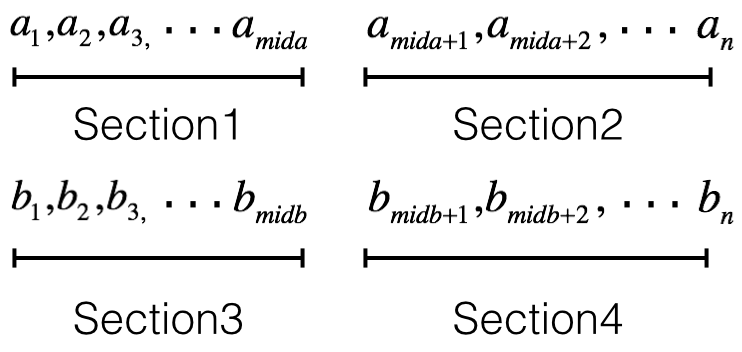
\includegraphics[scale=0.4]{hw2p3}
\caption{Picture of putting balls into bins}
\label{fig:p3}
\end{figure}

where $mida$ is the mid index of the first array $A$ and $midb$ is the mid index of the second array $B$. \\

If $mida + midb < k^{*}$, then it means that the $k^*$ smallest element is at \{Section1, Section2, Section4\} or \{Section2, Section3, Section4\}, the reason is as follows. If $A[mida] > B[midb]$, we can safely discard section3 since every element of section3 is smaller than $A[mida]$ and cannot be the $k^{*}$th smallest element of the union array. Similarly, If $A[mida] < B[midb]$ then we can discard section1.\\

However, if $mida + midb > k^{*}$, then it means that the $k^*$ smallest element is at \{Section1, Section2, Section3\} or \{Section1, Section3, Section4\}, the reason is as follows. If $A[mida] < B[midb]$, we can safely discard section4 since every element of section4 is bigger than $A[mida]$ and cannot be the $k^{*}$th smallest element of the union array. Similarly, If $A[mida] > B[midb]$ then we can discard section2.\\

The pseudo code is as follows:
\begin{algorithm}
\caption{Find($A$, $B$, $k^{*}$), $k^{*} = n - k + 1$}\label{euclid}
\begin{algorithmic}
\If {\textit{length(A)} = 0} \Return $B[k^{*}]$
\EndIf
\If {\textit{length(B)} = 0} \Return $A[k^{*}]$
\EndIf
\State $mida \gets length(A)/2$
\State $midb \gets length(B)/2$
\If {$mida + midb < k^{*}$} 
	\If {$A[mida] > B[midb]$}  $Find(A, B[midb + 1:], k^{*} - midb - 1)$
	\Else  $Find(A[mida + 1:], B, k^{*} - mida - 1)$
	\EndIf
\Else 
	\If {$A[mida] > B[midb]$}  $Find(A[:mida], B, k^{*})$
	\Else  $Find(A, B[:midb], k^{*})$
	\EndIf
\EndIf
\end{algorithmic}
\end{algorithm}

Since we halved the search space of A and B in each iteration, so the time complexity is $O(logn + logn) = O(logn)$
\section{Problem IV}

\begin{enumerate}[label=(\alph*)]
	\item \textbf{proof:} \\
	To show the rank of the root is $O(logn)$, we could first alternatively show that total nodes of a leftist heap with length of the rank of root is $k$ is at least $2^{k + 1} - 1$.\\

	By induction on the height $h$ of the give leftist heap $L$.\\

	Basis ($h=0$): Then $L$ consists of a single node and its right path has length $k=0$. Indeed, $L$ has $1 \geq 2^{1} - 1$ nodes, as wanted.\\

	\textit{Inductive Step} ($h>0$): Suppose the theorem holds for all leftist heaps that have height $< h$ and let $L$ be a leftist heap of height $h$. Further, let $k$ be the length of $L$'s right path and $n$ be the number of nodes in $L$. Consider two cases:\\

	\textit{Case 1}: $k=0$ (i.e. $L$ has no right subtree). But then clearly $n \geq 1 = 2^1 - 1$ as wanted.\\

	\textit{Case 2}: $k>0$. Let $L_L$, $L_R$ be the left and right subtrees of $L$; $n_L$, $n_R$ be the number of nodes in $L_L$ and $L_R$; and $k_L$, $k_R$ be the lengths of the right paths in $L_L$ and $L_R$ respectively. Because the left and right subtrees of a leftist heap are leftist heaps and the distance of a leftist heap's root is equal to the length of the tree's right path. Then we have $k_R = k - 1$, and by definition of leftist heap $k_L \geq k_R$. Since $L_L$, $L_R$ have height < $h$ we get, by induction hypothesis, $n_R \geq 2^k - 1$ and $n_L \geq 2^k - 1$. But $n = n_L + n_R +1$ and thus, $n \geq 2^k - 1 + 2^k - 1 + 1 =2^{k+1} - 1$. Therefore $n \geq 2^{k+1} - 1$, as wanted. Because $k = rank(x)$, we have
	\begin{align*}
	n &\geq 2^{rank(x) + 1} - 1\\
	n + 1 &\geq 2^{rank(x) + 1}\\
	log(n + 1) &\geq rank(x) + 1\\
	rank(x) &\leq lg(n + 1) - 1 = O(logn) 
	\end{align*}

	\item \textbf{Solution:} \\
	If one of the two leftist heap is empty, we are done. Otherwise we want to merge two non-empty leftist heaps $h_1$ and $h_2$. We can assume that without loss of generality, that the key in the root of $h_1$ is less than or equal to the key in the root of $h_2$. If $key(h_1) > key(h_2)$ we swap $h_1$ and $h_2$, so $h_1$ has the smaller root. Recursively we merge $h_2$ with the right subtree of $h_1$, and we make the resulting leftist tree into the right subtree of $h_1$. The pseudo code below gives more details. 
	\begin{algorithm}
	\caption{MERGE($h_1$, $h_2$)}\label{euclid}
	\begin{algorithmic}
	\If {$h_1  = \phi$} \Return $h_2$
	\ElsIf {$h_2 = \phi$} \Return $h_1$
	\Else
		\If {$key(h_1) > key(h_2)$} 
		\State $swap(h_1, h_2)$
		\EndIf
		$right(h_1) \gets MERGE(right(h_1), h_2) $ \\
		// merge $h_2$ on right 
		% \If {$rightChildOf(h_1) \neq \phi$ \textbf{and} ($leftChildOf(h_1) = \phi$ \textbf{or} $rank(rightChildOf(h_1)$) > $rank(leftChildOf(h_2)$))} 
		% \State $swap(rightChildOf(h_1), leftChildOf(h_1))$ \\
		% // swap children to make leftist \\
		% \EndIf
		% \If {$rightChildOf(h_1) = \phi$} 
		% \State $rank(h_1) = 0$
		% \Else
		% \State $rank(h_1) \gets rank(rightChildOf(h_1)) + 1$ \\
		% // update rank value \\
		% \EndIf
		% \Return $h_1$
	\EndIf
	\State \textbf{end} MERGE
	\end{algorithmic}
	\end{algorithm}
	The complexity of the algorithm is proportional to the number of recursive calls to MERGE.  It is easy to see that, in the worst case, this will be equal to rank of $h_1$'s root plus rank of $h_2$'s root. Let the number of nodes in these trees be $n_1$ and $n_2$. By the proof procedure in question(a), we have $rank(h_1) \leq log(n_1)$, and $rank(h_2) \leq log(n_2)$. Thus $rank(h_1) + rank(h_2) \leq logn_1 + logn_2$. Let $n$ = max($n_1$, $n_2$). Then $rank(h_1) + rank(h_2) \leq 2logn$. Therefore, MERGE is called at most $2logn$ times, and the complexity of the algorithm is $O(log(n)$ in the worst case. \\

	Meanwhile, because we maintain the key($h_1$) is smaller than key($h_2$) by swapping $h_1$ and $h_2$ if $key(h_1) < key(h_2)$ and then we let the $right(h_1)$ equals to the merge result of $right(h_1)$ and $h_2$. So we will always let the node with smaller key merge earlier than the node with larger key. That is, the order invariant is maintained. 

	\item \textbf{Solution:} \\
	We can suppose that $x$ is not on the rightmost path of the given leftist heap and the rank of $x$ changed after MERGE operation. Since every MERGE operation happens on the right child of every node, so for those node not on the right most path will still follow $rank(x) = 1 + rank(right(x))$ without any changes with their rank in the new merged tree which is a contradiction.\\

	So, the rank of a node $x$ might change if and only if $x$ is on the rightmost path.

	\item \textbf{Solution:} \\
	Similar with the process in question($b$), if one of the two leftist heap is empty, we are done. Otherwise we want to merge two non-empty leftist heaps $h_1$ and $h_2$. We can assume that without loss of generality, that the key in the root of $h_1$ is less than or equal to the key in the root of $h_2$. If $key(h_1) > key(h_2)$ we swap $h_1$ and $h_2$, so $h_1$ has the smaller root. Recursively we merge $h_2$ with the right subtree of $h_1$, and we make the resulting leftist tree into the right subtree of $h_1$. If this has made the rank of the right subtree's root longer than the rank of the left subtree's root, we simply interchange the left and right children of $h_1$'s root(thereby making what used to be the right subtree of $h_1$ into its left subtree and vice-versa). Finally, we update the rank of $h_1$'s root . The pseudo code below gives more details. 
	\begin{algorithm}
	\caption{MERGE($h_1$, $h_2$)}\label{euclid}
	\begin{algorithmic}
	\If {$h_1  = \phi$} \Return $h_2$
	\ElsIf {$h_2 = \phi$} \Return $h_1$
	\Else
		\If {$key(h_1) > key(h_2)$} 
		\State $swap(h_1, h_2)$
		\EndIf
		$right(h_1) \gets MERGE(right(h_1), h_2) $ \\
		// merge $h_2$ on right and swap if needed \\
		\If {$right(h_1) \neq \phi$ \textbf{and} ($left(h_1) = \phi$ \textbf{or} $rank(right(h_1)$) > $rank(left(h_2)$))} 
		\State $swap(right(h_1), left(h_1))$ \\
		// swap children to make leftist \\
		\EndIf
		\If {$right(h_1) = \phi$} 
		\State $rank(h_1) = 0$
		\Else
		\State $rank(h_1) \gets rank(right(h_1)) + 1$ \\
		// update rank value \\
		\EndIf
		\Return $h_1$
	\EndIf
	\State \textbf{end} MERGE
	\end{algorithmic}
	\end{algorithm}

	The order invariant is maintained which is proved in question($b$). As shown in the pseudo code above, we can note that if node $x$ with $rank(left(x)) < rank(right(x))$, then its children $left(x)$ and $right(x)$ will be swapped in updating which guarantees the balance invariant.\\

	The running time analysis is pretty similar with question($b$), observe that there is a constant number of steps that must be executed before and after each recursive call to MERGE. Thus the complexity of the algorithm is proportional to the number of recursive calls to MERGE.  It is easy to see that, in the worst case, this will be equal to rank of $h_1$'s root plus rank of $h_2$'s root. Let the number of nodes in these trees be $n_1$ and $n_2$. By the proof procedure in question(a), we have $rank(h_1) \leq log(n_1)$, and $rank(h_2) \leq log(n_2)$. Thus $rank(h_1) + rank(h_2) \leq logn_1 + logn_2$. Let $n$ = max($n_1$, $n_2$). Then $rank(h_1) + rank(h_2) \leq 2logn$. Therefore, MERGE is called at most $2logn$ times, and the complexity of the algorithm is $O(log(n)$ in the worst case. \\

	\item \textbf{Solution:} \\
	Using the MERGE algorithm in problem(b) we can write algorithm for Insert and DeleteMin:\\

	Insert($e$, $r$) where $e$ is an element, $r$ is the root of the given leftist heap.\\

	1. Let $r'$ be a the leftist heap containing only $e$.\\
	2. MERGE($r'$, $r$).\\

	As is described above, we could treat the element we want to insert to the given leftist heap as a leftist heap contains only one element as root node. Then we could merge this leftist heap with the given leftist heap as we did before. The running time of merging and rank updates is $O(logn)$ as we discussed in previous steps.\\

	DeleteMin($r$)\\

	1. $min$ $\gets$ element stored at $r$ (root of the given leftist heap)\\
	2. $r \gets MERGE(left(r), right(r))$\\
	3. \textbf{return} $min$.\\

	To delete the minimum element in the give leftist heap, we can start with removing the root of the given leftist heap. Then, we could merge and update the rank of its left and right subtrees, which has a running time of $O(logn)$ as we discussed above. 

\end{enumerate}

\end{document}